\section{Uvod}
Video nadzor se danas uvelike koristi u velikom broju raznih područja kao na primjer sigurnost, medicina, transport
i brojni drugi.
\paraBreak
Zbog naglog usvajanja interneta proteklih godina, većina nadzornih sustava, takozvani "pametni" uređaji, oslanjaju se
na komunikaciju putem istog. \\
Tradicionalni nadzorni sustav sastoji se od naravno od kamere, neke vrste prijenosnog kabla koji povezuje kameru sa
računalom te video nadzorne platforme odnosno aplikacijom. Ovaj radi se primarno bavi implementacijom aplikacijskog djela a 
za sklopovski dio koristi Raspberry pi platformu.
\paraBreak
Video nadzor možemo generalno podijeliti na dvije vrste, pasivni nadzor i nadzor u realnom vremenu. \\
Kod pasivnog nadzora nije moguće u bilo kojem trenutku vidjeti prikaz kamere, video se sprema na neku vrstu spremišta, bilo
lokalno kao tvrdi disk ili 
\foreign{cloud}
\footnote
{
  Aplikacije ili softver uvijek dostupni putem interneta, na poslužiteljima treće strane, obično se iznajmljuju na neki ne nužno
  određen period vremena 
}
rješenje. \\
Nadzor u realnom vremenu kao što i ime sugerira omogućuje pregled u bilo kojem trenutku, ali najčešće i pohranjuje
video na isti način kao i pasivni. \\
Implementacija ovog rada spada pod nadzor u realnom vremenu, ali na nikakav način ne pohranjuje snimani video, zbog pre velikih
troškova koje takva pohrana nosi. 
\paraBreak
Svrhe ovakvih pametnih nadzora su brojne, ali osim očitih, zbog velikog napretka računalnih mreža, procesiranja digitalnih
slika i načina prijenosa podataka relativno je lako doći do robusnih i pametnih implementacija koje koriste strojno učenje
za prepoznavanje događaja koje je odredio korisnik. Takvi nadzorni sustavi imaju ogroman potencijal i integraciju sa virtualno
bilo kojim uređajem koji ima pristup internetu. Kao demonstraciju u sklopu ovog rada implementiran je poslužitelj
koji je sposoban prenositi nadzorni video velikom broju uređaja pod uvjetom da su spojeni na internet.

\pagebreak
\subsection{Raspberry pi}
Raspberry pi je serija malih \foreign{single-board \footnote{Računalo u potpunosti izgrađeno na jednoj pločici}} 
računala široko korištenih u svrhe eksperimentalnih projekata. \cite{rPiBook}
\paraBreak
Idealan je za tu upotrebu zbog privlačne cijene i odlične portabilnosti te jako male potrošnje struje.
\paraBreak
Za ovaj rad je odabran zbog osim navedenih razloga još i radi ogromnog izbora eksternih modula, specifično službenog kamera modula
koji služi kao baza cijelog projekta.

\begin{figure}[ht]
  \centering
  \begin{subfigure}{.5\textwidth}
    \centering
    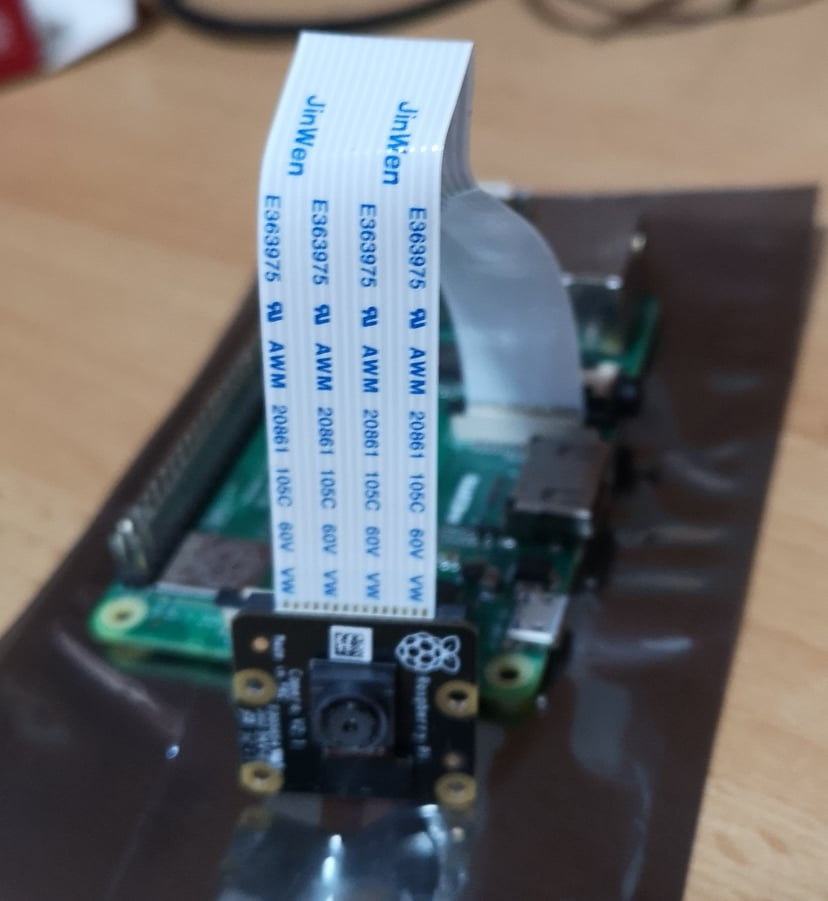
\includegraphics[width=0.95\textwidth]{raspberyy-pi-camera.jpg}
    \caption{Kamera modul}
  \end{subfigure}%
  \begin{subfigure}{.5\textwidth}
    \centering
    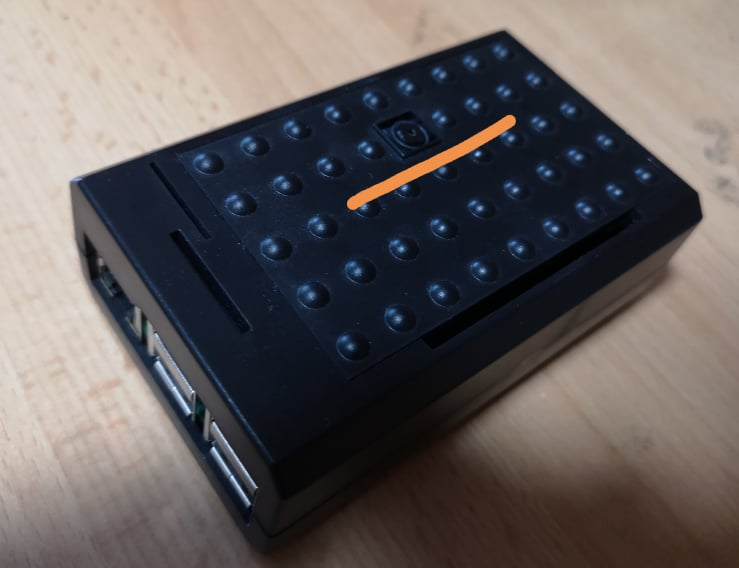
\includegraphics[height=7.6cm, width=0.95\textwidth]{raspberyy-pie-in-box.jpg}
    \caption{Kutija sa otvorom za leću kamere}
  \end{subfigure}%
  \caption{Raspberry pi dodaci}
\end{figure}

\clearpage
\subsection{Biblioteka za obradu videa} \label{sec:ffmpeg}
  \foreign{FFmpeg} je 
  \footnote
  {
    Projekti koji otvoreno dozvoljavaju korištenje istih ovisno o licensama, te koji imaju javno dostupan izvorni kod
    i najčešće se oslanjaju na zajednicu programera na daljnjem razvoju.
  }
  {\foreign{open-source}} 
  projekt koji se sastoji od mnoštva biblioteka za manipuliranje videom, audiom i ostalom multimedijom.
  \cite{ffmpegBook}
\paraBreak
Najveća primjena mu je u transkodiranju, editiranju, skaliranju i raznim efektima videa.
\paraBreak
Najbitnije biblioteke iz FFmpeg-a koje se koriste u ovom radu su \cite{ffmpegDocs}
\begin{itemize}
  \item libavcodec - audio/video kodek biblioteka
  \item libavformat - audio/video kontejner \hyperref[sct:mux]{\foreign{}{mux}} i \hyperref[sct:demux]{\foreign{}{demux}} biblioteka
  \item libavdevice - biblioteka za dohvaćanje i rad dostupnim multimedija uređajima
  \item libswscale - biblioteka za manipulaciju i skaliranje slika videa
\end{itemize}
Koristi se u mnogim popularnim projektima kao što su Google Chrome, VLC Player, YouTube, Blender, HandBrake, Kodi, Plex. \cite{ffmpegBook}
